% Options for packages loaded elsewhere
\PassOptionsToPackage{unicode}{hyperref}
\PassOptionsToPackage{hyphens}{url}
%
\documentclass[
  ignorenonframetext,
  aspectratio=141,
]{beamer}
\usepackage{pgfpages}
\setbeamertemplate{caption}[numbered]
\setbeamertemplate{caption label separator}{: }
\setbeamercolor{caption name}{fg=normal text.fg}
\beamertemplatenavigationsymbolsempty
% Prevent slide breaks in the middle of a paragraph
\widowpenalties 1 10000
\raggedbottom

\usepackage{amsmath,amssymb}
\usepackage{iftex}
\ifPDFTeX
  \usepackage[T1]{fontenc}
  \usepackage[utf8]{inputenc}
  \usepackage{textcomp} % provide euro and other symbols
\else % if luatex or xetex
  \usepackage{unicode-math}
  \defaultfontfeatures{Scale=MatchLowercase}
  \defaultfontfeatures[\rmfamily]{Ligatures=TeX,Scale=1}
\fi
\usepackage{lmodern}
\usetheme[]{CambridgeUS}
\usecolortheme{dolphin}
\usefonttheme{structurebold}
\ifPDFTeX\else  
    % xetex/luatex font selection
\fi
% Use upquote if available, for straight quotes in verbatim environments
\IfFileExists{upquote.sty}{\usepackage{upquote}}{}
\IfFileExists{microtype.sty}{% use microtype if available
  \usepackage[]{microtype}
  \UseMicrotypeSet[protrusion]{basicmath} % disable protrusion for tt fonts
}{}
\makeatletter
\@ifundefined{KOMAClassName}{% if non-KOMA class
  \IfFileExists{parskip.sty}{%
    \usepackage{parskip}
  }{% else
    \setlength{\parindent}{0pt}
    \setlength{\parskip}{6pt plus 2pt minus 1pt}}
}{% if KOMA class
  \KOMAoptions{parskip=half}}
\makeatother
\usepackage{xcolor}
\newif\ifbibliography
\setlength{\emergencystretch}{3em} % prevent overfull lines
\setcounter{secnumdepth}{-\maxdimen} % remove section numbering


\providecommand{\tightlist}{%
  \setlength{\itemsep}{0pt}\setlength{\parskip}{0pt}}\usepackage{longtable,booktabs,array}
\usepackage{calc} % for calculating minipage widths
\usepackage{caption}
% Make caption package work with longtable
\makeatletter
\def\fnum@table{\tablename~\thetable}
\makeatother
\usepackage{graphicx}
\makeatletter
\def\maxwidth{\ifdim\Gin@nat@width>\linewidth\linewidth\else\Gin@nat@width\fi}
\def\maxheight{\ifdim\Gin@nat@height>\textheight\textheight\else\Gin@nat@height\fi}
\makeatother
% Scale images if necessary, so that they will not overflow the page
% margins by default, and it is still possible to overwrite the defaults
% using explicit options in \includegraphics[width, height, ...]{}
\setkeys{Gin}{width=\maxwidth,height=\maxheight,keepaspectratio}
% Set default figure placement to htbp
\makeatletter
\def\fps@figure{htbp}
\makeatother
% definitions for citeproc citations
\NewDocumentCommand\citeproctext{}{}
\NewDocumentCommand\citeproc{mm}{%
  \begingroup\def\citeproctext{#2}\cite{#1}\endgroup}
\makeatletter
 % allow citations to break across lines
 \let\@cite@ofmt\@firstofone
 % avoid brackets around text for \cite:
 \def\@biblabel#1{}
 \def\@cite#1#2{{#1\if@tempswa , #2\fi}}
\makeatother
\newlength{\cslhangindent}
\setlength{\cslhangindent}{1.5em}
\newlength{\csllabelwidth}
\setlength{\csllabelwidth}{3em}
\newenvironment{CSLReferences}[2] % #1 hanging-indent, #2 entry-spacing
 {\begin{list}{}{%
  \setlength{\itemindent}{0pt}
  \setlength{\leftmargin}{0pt}
  \setlength{\parsep}{0pt}
  % turn on hanging indent if param 1 is 1
  \ifodd #1
   \setlength{\leftmargin}{\cslhangindent}
   \setlength{\itemindent}{-1\cslhangindent}
  \fi
  % set entry spacing
  \setlength{\itemsep}{#2\baselineskip}}}
 {\end{list}}
\usepackage{calc}
\newcommand{\CSLBlock}[1]{\hfill\break\parbox[t]{\linewidth}{\strut\ignorespaces#1\strut}}
\newcommand{\CSLLeftMargin}[1]{\parbox[t]{\csllabelwidth}{\strut#1\strut}}
\newcommand{\CSLRightInline}[1]{\parbox[t]{\linewidth - \csllabelwidth}{\strut#1\strut}}
\newcommand{\CSLIndent}[1]{\hspace{\cslhangindent}#1}

\usepackage{booktabs}
\usepackage{longtable}
\usepackage{array}
\usepackage{multirow}
\usepackage{wrapfig}
\usepackage{float}
\usepackage{colortbl}
\usepackage{pdflscape}
\usepackage{tabularx}
\usepackage{xltabular}
\usepackage{threeparttable}
\usepackage{threeparttablex}
\usepackage[normalem]{ulem}
\usepackage{makecell}
\usepackage{xcolor}
\setbeamertemplate{items}[circle]
\usepackage{setspace}
\usepackage{booktabs}
\usepackage{amsmath}
\setbeamerfont{title}{size=\Large}
\setbeamerfont{author}{size=\large}
\setbeamerfont{subtitle}{size=\large}
\setbeamerfont{institute}{size=\small}
\setbeamerfont{date}{size=\small}
\useoutertheme[footline=authorinstitute,subsection=false]{miniframes}
\setbeamerfont{section in head/foot}{size=\tiny}
\setbeamersize{mini frame size=.08cm, mini frame offset=.02cm}
\setbeamersize{text margin left=0.6cm, text margin right=0.6cm}
\definecolor{UBCblue}{rgb}{0.04706, 0.13725, 0.26667}
\usecolortheme[named=UBCblue]{structure}
\setbeamertemplate{frametitle}[default][center]
\setbeamerfont{frametitle}{size=\large}
\setbeamertemplate{frame numbering}{}
\usepackage{appendixnumberbeamer}
\let\oldsection\section
\renewcommand{\section}{\ifnum\value{section}=5 \appendix\fi\oldsection}
\makeatletter
\@ifpackageloaded{caption}{}{\usepackage{caption}}
\AtBeginDocument{%
\ifdefined\contentsname
  \renewcommand*\contentsname{Table of contents}
\else
  \newcommand\contentsname{Table of contents}
\fi
\ifdefined\listfigurename
  \renewcommand*\listfigurename{List of Figures}
\else
  \newcommand\listfigurename{List of Figures}
\fi
\ifdefined\listtablename
  \renewcommand*\listtablename{List of Tables}
\else
  \newcommand\listtablename{List of Tables}
\fi
\ifdefined\figurename
  \renewcommand*\figurename{Figure}
\else
  \newcommand\figurename{Figure}
\fi
\ifdefined\tablename
  \renewcommand*\tablename{Table}
\else
  \newcommand\tablename{Table}
\fi
}
\@ifpackageloaded{float}{}{\usepackage{float}}
\floatstyle{ruled}
\@ifundefined{c@chapter}{\newfloat{codelisting}{h}{lop}}{\newfloat{codelisting}{h}{lop}[chapter]}
\floatname{codelisting}{Listing}
\newcommand*\listoflistings{\listof{codelisting}{List of Listings}}
\makeatother
\makeatletter
\makeatother
\makeatletter
\@ifpackageloaded{caption}{}{\usepackage{caption}}
\@ifpackageloaded{subcaption}{}{\usepackage{subcaption}}
\makeatother
\ifLuaTeX
  \usepackage{selnolig}  % disable illegal ligatures
\fi
\usepackage{bookmark}

\IfFileExists{xurl.sty}{\usepackage{xurl}}{} % add URL line breaks if available
\urlstyle{same} % disable monospaced font for URLs
\hypersetup{
  pdftitle={Decomposing Exchange Rate Responses to News: Evidence from South Africa},
  hidelinks,
  pdfcreator={LaTeX via pandoc}}

\title{Decomposing Exchange Rate Responses to News: Evidence from South
Africa}
\author{Xolani Sibande \and Ozer Karagedikli}
\date{}
\institute{South Africa Reserve Bank}

\begin{document}
\frame{\titlepage}

\section{Introduction}\label{introduction}

\begin{frame}{Motivation}
\phantomsection\label{motivation}
\begin{itemize}
\tightlist
\item
  Monetary policy news moves exchange rates, but \textbf{how} is less
  clear for small open economies
\item
  Textbook channel: a tightening raises the domestic interest rate gap,
  and the currency appreciates
\item
  In practice, the link is weak and unstable: currencies also respond to
  risk premia and global conditions
\item
  South Africa is a useful case: an open, inflation-targeting economy
  with a liquid, freely floating currency
\item
  High-frequency identification of policy surprises lets us isolate the
  news component (Kuttner 2001; Cook and Hahn 1989; Gurkaynak, Sack, and
  Swanson 2005; Swanson 2021; Miranda-Agrippino and Ricco 2021)
\end{itemize}
\end{frame}

\begin{frame}{Typical moves on announcement days}
\phantomsection\label{typical-moves-on-announcement-days}
\begin{table}[!h]
\centering\begingroup\fontsize{9}{11}\selectfont

\resizebox{\ifdim\width>\linewidth\linewidth\else\width\fi}{!}{
\begin{tabular}[t]{lrrrr}
\toprule
Sample & Days & Spot: mean move (\%) & Spot: days over 1\% & 2y gap: mean move (bp)\\
\midrule
Other days & 3,633 & 0.82 & 30\% & 5.5\\
SA monetary policy & 101 & 0.88 & 33\% & 9.8\\
SA data releases & 424 & 0.90 & 35\% & 7.3\\
US monetary policy & 123 & 1.13 & 50\% & 7.7\\
\bottomrule
\end{tabular}}
\endgroup{}
\end{table}

\vspace{0.2cm}

\begin{itemize}
\tightlist
\item
  On an ordinary day the rand moves about 0.8\%, and on SA monetary
  policy and data release days it moves about the same (0.88\% and
  0.90\%)
\item
  US monetary policy days stand out: 1.13\% on average, with 50\% of
  days moving more than 1\%
\item
  The rate gap reacts more clearly on SA monetary policy days: about 10
  bp at the 2y, against 6 bp on other days
\item
  The news is a small signal against the rand's everyday volatility, so
  we need to isolate the surprise
\end{itemize}

\footnotesize Mean move is the mean absolute daily change. Other days
have no announcement.
\end{frame}

\begin{frame}{Related literature: exchange rate responses to news}
\phantomsection\label{related-literature-exchange-rate-responses-to-news}
\begin{itemize}
\tightlist
\item
  Macro announcement surprises cause jumps in exchange rates in
  high-frequency data (Andersen et al. 2003)
\item
  The joint response of exchange rates and term structures is read
  through uncovered interest parity and risk premia: a
  stronger-than-expected release can appreciate the dollar while
  implying overshooting (Faust et al. 2003)
\item
  Small open economies: an unanticipated 25 bp tightening appreciates
  the exchange rate by about 0.35\% on average, yet policy accounts for
  only a small share of exchange rate variability (Kearns and Manners
  2005; Zettelmeyer 2004)
\item
  New Zealand: data and monetary policy surprises have large effects,
  and the published rate track adds about 10\% explanatory power
  (Karagedikli and Siklos 2008)
\end{itemize}
\end{frame}

\begin{frame}{Closest in design to ours}
\phantomsection\label{closest-in-design-to-ours}
\begin{itemize}
\tightlist
\item
  Coleman and Karagedikli (2012) compare the response of the spot rate,
  2y and 5y swap rate differentials and the synthetic forward schedule
  in New Zealand
\item
  Monetary surprises move spot and the 5y swap rate by similar amounts,
  so forwards respond little
\item
  CPI and GDP surprises move spot about three times as much as the 5y
  rate, so forwards appreciate on stronger CPI or GDP news
\item
  This contrasts with standard theory and US evidence
\item
  We ask the same questions for South Africa, with forwards implied by
  CIP (see appendix)
\end{itemize}
\end{frame}

\begin{frame}{Related literature: theory, term structure and information
effects}
\phantomsection\label{related-literature-theory-term-structure-and-information-effects}
\begin{itemize}
\tightlist
\item
  Exchange rates and fundamentals: fundamentals help little in
  predicting floating exchange rates, which look close to a random walk
  (Engel and West 2005; Engel et al. 2007)
\item
  Interest rate rules link monetary policy to the real exchange rate
  (Engel and West 2004)
\item
  What the exchange rate response to inflation news says about monetary
  policy (Clarida and Waldman 2008)
\item
  Term structure responses to economic and monetary policy surprises
  (Gürkaynak, Sack, and Swanson 2005)
\item
  Information effects: how forward guidance is worded shapes private
  sector responses (Lunsford 2020; Jarociński 2024), which motivates the
  CBI factor
\end{itemize}
\end{frame}

\begin{frame}{What we add}
\phantomsection\label{what-we-add}
\begin{itemize}
\tightlist
\item
  Four monetary policy factors for South Africa: Target, FG, CBI and
  country risk, plus data releases and US surprises
\item
  Responses across the term structure up to 10 years, in spot and the
  SA--US OIS rate gap
\item
  A split of the rate gap into a news-driven (predictable) and a
  non-news (unpredictable) part, each related to the rand
\item
  Local projections that show whether a surprise shifts the gap curve in
  parallel or tilts it
\end{itemize}
\end{frame}

\begin{frame}{What we ask}
\phantomsection\label{what-we-ask}
\begin{enumerate}
\tightlist
\item
  How do the rand and the SA--US interest rate gap respond to South
  African monetary policy surprises and to data releases?
\item
  Does the rand respond to the \textbf{news-driven} part of the rate
  gap, or to the rest?
\item
  Do US monetary policy surprises work through the same channel?
\end{enumerate}
\end{frame}

\section{Data and methodology}\label{data-and-methodology}

\begin{frame}{Data and sample}
\phantomsection\label{data-and-sample}
\begin{table}[!h]
\centering\begingroup\fontsize{9}{11}\selectfont

\resizebox{\ifdim\width>\linewidth\linewidth\else\width\fi}{!}{
\begin{tabular}[t]{lrr}
\toprule
Data & Event days & Sample\\
\midrule
SA monetary policy surprises (Pirozhkova et al. 2024) & 101 & Apr 2008 -- Nov 2024\\
SA data releases (CPI, GDP, unemployment) & 424 & Oct 2007 -- Dec 2024\\
US monetary policy surprises (Jarociński 2024) & 123 & Oct 2007 -- Sep 2024\\
ZARONIA and US OIS rates & Daily & \\
ZAR/USD spot rate & Daily & \\
\bottomrule
\end{tabular}}
\endgroup{}
\end{table}

\vspace{0.3cm}

\begin{itemize}
\tightlist
\item
  Regressions use event days only; the SA sample ends in 2024 because of
  ZARONIA data availability
\end{itemize}
\end{frame}

\begin{frame}{Four surprise factors}
\phantomsection\label{four-surprise-factors}
\begin{itemize}
\tightlist
\item
  \textbf{Target}: the immediate market reaction to the policy rate
  decision
\item
  \textbf{Forward guidance (FG)}: the response to the communicated
  longer-term path of policy
\item
  \textbf{Central bank information (CBI)}: what the announcement reveals
  about the central bank's view of the economy (Jarociński 2024)
\item
  \textbf{Country risk (CR)}: the central bank's role in responding to
  external shocks in a small open economy (Pirozhkova, Ricco, and Viegi
  2024)
\item
  US surprises are defined in the same way, with an added large-scale
  asset purchase (LSAP) factor and no CR factor
\item
  Data release surprises: \textbf{actual minus the median analyst
  forecast}
\end{itemize}
\end{frame}

\begin{frame}{Variables and units}
\phantomsection\label{variables-and-units}
\begin{table}[!h]
\centering\begingroup\fontsize{9}{11}\selectfont

\resizebox{\ifdim\width>\linewidth\linewidth\else\width\fi}{!}{
\begin{tabular}[t]{lll}
\toprule
Variable & Definition & Unit\\
\midrule
Surprises & Policy factors and release surprises & pp\\
Spot & Daily log change in ZAR/USD & \% (positive = rand depreciates)\\
OIS gap, tenor n & Change in (SA OIS - US OIS) & pp\\
Forward, tenor n & Spot change + n x change in OIS gap & \%\\
\bottomrule
\end{tabular}}
\endgroup{}
\end{table}

\vspace{0.3cm}

\begin{itemize}
\tightlist
\item
  Coefficients read as: the response to a \textbf{1 pp} surprise
\item
  Tenors: 1, 2, 3, 4, 5 and 10 years
\end{itemize}
\end{frame}

\begin{frame}{How the rate gap relates to the rand}
\phantomsection\label{how-the-rate-gap-relates-to-the-rand}
\(S\) is ZAR per USD (a rise is a weaker rand). The gap is the SA minus
US OIS rate at tenor \(n\):

\begin{equation}\phantomsection\label{eq-gap}{\text{gap}_t^{(n)} = r_t^{SA,(n)} - r_t^{US,(n)}}\end{equation}

\begin{itemize}
\tightlist
\item
  \textbf{CIP:} the forward premium equals the gap,
  \(\ln F^{(n)} - \ln S \approx n \times \text{gap}^{(n)}\). This ties
  the gap to the forward, not to spot
\item
  \textbf{UIP:} the expected rand depreciation equals the gap.
  Rearranged, with a risk premium \(rp_t\) that is zero under UIP:
\end{itemize}

\begin{equation}\phantomsection\label{eq-uip}{\ln S_t = E_t[\ln S_{t+n}] - n \times \text{gap}_t^{(n)} + rp_t}\end{equation}

\begin{itemize}
\tightlist
\item
  A surprise that raises the gap lowers spot today: the rand appreciates
  by up to \(n \times \Delta\text{gap}\) if the long-run rate is
  unchanged, then drifts weaker (overshooting)
\item
  UIP fails in practice, and a surprise can also shift the long-run rate
  or the risk premium, so the sign and size of the response are an
  empirical question (Faust et al. 2003)
\end{itemize}
\end{frame}

\begin{frame}{Forward rates are implied by the rate gap}
\phantomsection\label{forward-rates-are-implied-by-the-rate-gap}
Covered interest parity links spot, forwards and the SA--US rate gap:

\begin{equation}\phantomsection\label{eq-forward}{\Delta \ln F_t^{(n)} = \Delta \ln S_t + n \, \Delta\left(r_t^{SA} - r_t^{US}\right)}\end{equation}

\begin{itemize}
\tightlist
\item
  Our forwards are constructed this way, so they carry no information
  beyond \textbf{spot and the rate gap}
\item
  The focus is therefore on spot and the gap; forwards translate the gap
  response into exchange-rate terms
\item
  Multiplying by the tenor makes long forwards mechanically more
  sensitive than short ones
\end{itemize}
\end{frame}

\begin{frame}{Event-study regressions}
\phantomsection\label{event-study-regressions}
\begin{equation}\phantomsection\label{eq-event}{\Delta y_t = \alpha + \beta \, s_t + \varepsilon_t}\end{equation}

\begin{itemize}
\tightlist
\item
  \(y_t\): spot or OIS gap at a given tenor (forwards are in the
  appendix)
\item
  \(s_t\): a monetary policy or data release surprise
\item
  Estimated on announcement or release days
\item
  Newey--West standard errors
\end{itemize}
\end{frame}

\begin{frame}{Splitting the rate gap into predictable and unpredictable
parts}
\phantomsection\label{splitting-the-rate-gap-into-predictable-and-unpredictable-parts}
Step 1: regress the change in the gap on the surprise

\begin{equation}\phantomsection\label{eq-first}{\Delta gap_t = \alpha + \gamma \, s_t + u_t}\end{equation}

\begin{itemize}
\tightlist
\item
  \textbf{Predictable} part: the fitted value (news-driven)
\item
  \textbf{Unpredictable} part: the residual
\end{itemize}

Step 2: relate each part to the exchange rate

\begin{equation}\phantomsection\label{eq-second}{\Delta spot_t = a + b_1 \, \widehat{gap}_t + b_2 \, \hat{u}_t + e_t}\end{equation}

Baseline: regress spot on the raw change in the gap
\end{frame}

\begin{frame}{Why split the gap into predictable and unpredictable
parts?}
\phantomsection\label{why-split-the-gap-into-predictable-and-unpredictable-parts}
\begin{itemize}
\tightlist
\item
  The gap moves for many reasons on an announcement day: the policy news
  itself, other news, risk sentiment and noise
\item
  \textbf{Predictable} part: the movement tied to the identified
  surprise, which is the interest rate channel that theory says should
  move the currency
\item
  \textbf{Unpredictable} part: everything else, including risk premia,
  information effects and noise. It is not clearly exogenous
\item
  Regressing spot on the raw gap mixes the two, so a real effect can be
  hidden
\item
  Using the predictable part is equivalent to an instrumental variable
  estimate with the surprise as the instrument. This assumes the
  surprise affects spot only through the gap, and it is unreliable when
  the gap barely responds to the surprise, as for Target and FG
\item
  Comparing the two parts shows whether the rand responds to expected
  interest rate differentials or to risk premia (Faust et al. 2003)
\end{itemize}
\end{frame}

\section{Results}\label{results}

\begin{frame}{SA monetary policy surprises: responses across variables}
\phantomsection\label{sa-monetary-policy-surprises-responses-across-variables}
\begin{center}
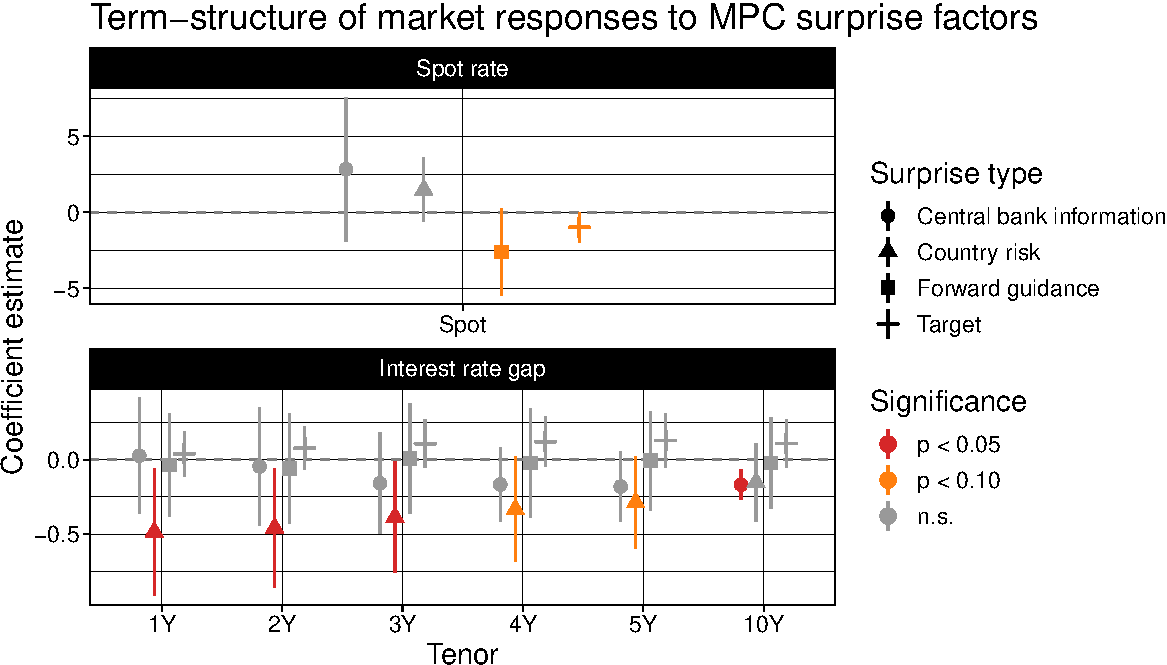
\includegraphics[width=1\textwidth,height=0.78\textheight]{exchange_rate_response_to_news_presentation_files/figure-beamer/mps-fig-1.pdf}
\end{center}
\end{frame}

\begin{frame}{SA monetary policy surprises: significant responses}
\phantomsection\label{sa-monetary-policy-surprises-significant-responses}
\begin{table}[!h]
\centering\begingroup\fontsize{9}{11}\selectfont

\resizebox{\ifdim\width>\linewidth\linewidth\else\width\fi}{!}{
\begin{tabular}[t]{llrrr}
\toprule
Surprise & Response & Coefficient & Std. error & p-value\\
\midrule
Target & Spot & -0.986* & 0.511 & 0.056\\
Forward Guidance & Spot & -2.603* & 1.452 & 0.076\\
Central Bank Information & OIS gap 10y & -0.168*** & 0.051 & 0.001\\
Country Risk & OIS gap 1y & -0.485** & 0.217 & 0.028\\
Country Risk & OIS gap 2y & -0.458** & 0.202 & 0.026\\
Country Risk & OIS gap 3y & -0.386** & 0.190 & 0.045\\
Country Risk & OIS gap 4y & -0.333* & 0.180 & 0.066\\
Country Risk & OIS gap 5y & -0.288* & 0.158 & 0.071\\
\bottomrule
\end{tabular}}
\endgroup{}
\end{table}

\vspace{0.2cm}

\footnotesize * p \textless{} 0.10, ** p \textless{} 0.05, *** p
\textless{} 0.01
\end{frame}

\begin{frame}{SA monetary policy surprises: what stands out}
\phantomsection\label{sa-monetary-policy-surprises-what-stands-out}
\begin{itemize}
\tightlist
\item
  A positive Target surprise is associated with rand appreciation: spot
  -0.99 (p = 0.056)
\item
  Forward guidance has the larger spot response: -2.60 (p = 0.076)
\item
  Both are only borderline significant (p \textless{} 0.10)
\item
  CBI lowers the long-end rate gap: 10y -0.17 (p = 0.001)
\item
  Country risk lowers the short-to-medium gap: 2y -0.46 (p = 0.026)
\item
  Most other responses are not distinguishable from zero in a sample of
  101 announcement days
\end{itemize}
\end{frame}

\begin{frame}{SA data releases}
\phantomsection\label{sa-data-releases}
\begin{center}
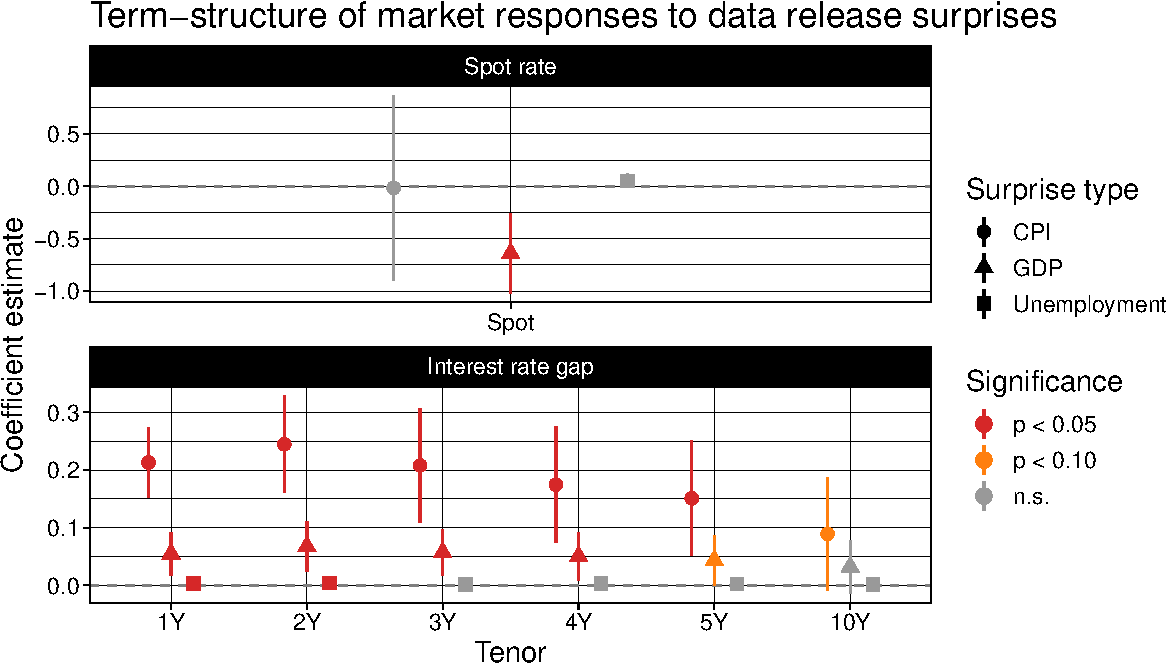
\includegraphics[width=1\textwidth,height=0.78\textheight]{exchange_rate_response_to_news_presentation_files/figure-beamer/releases-fig-1.pdf}
\end{center}
\end{frame}

\begin{frame}{SA data releases: what stands out}
\phantomsection\label{sa-data-releases-what-stands-out}
\begin{itemize}
\tightlist
\item
  Data releases move the rate gap more clearly than monetary policy
  surprises do
\item
  A CPI surprise raises the gap at all tenors: 2y 0.24 (p \textless{}
  0.001)
\item
  A GDP surprise strengthens the rand: spot -0.64 (p = 0.001), and also
  raises the short-to-medium gap
\item
  Unemployment has small effects on the gap at short tenors
\end{itemize}
\end{frame}

\begin{frame}{US monetary policy surprises}
\phantomsection\label{us-monetary-policy-surprises}
\begin{center}
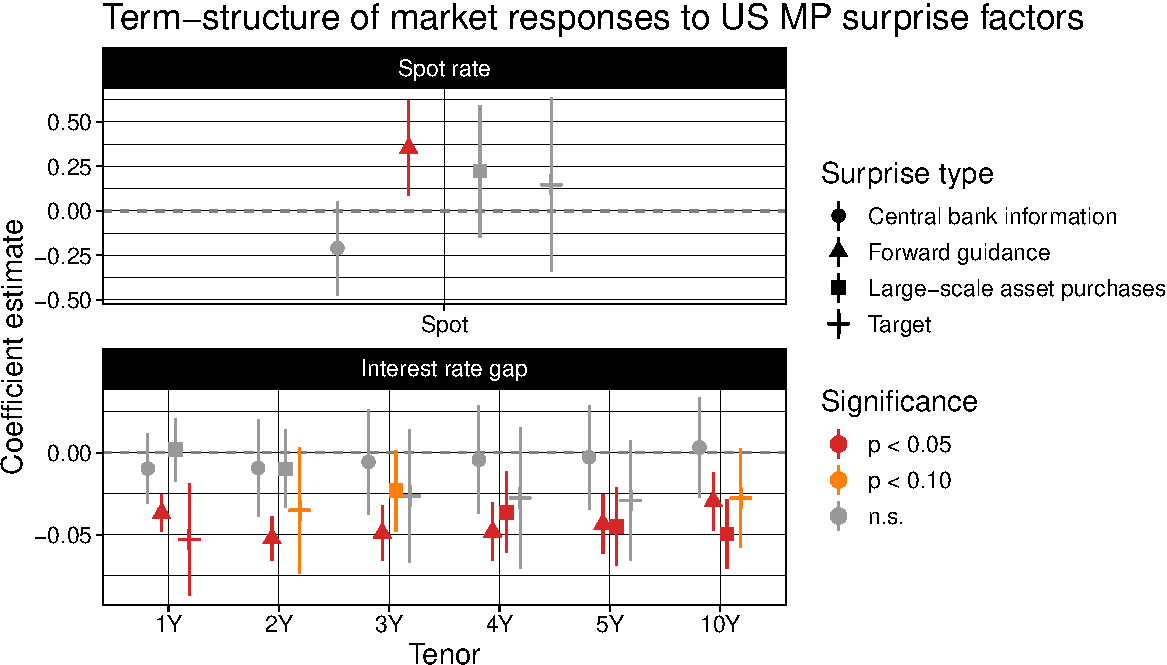
\includegraphics[width=1\textwidth,height=0.78\textheight]{exchange_rate_response_to_news_presentation_files/figure-beamer/us-fig-1.pdf}
\end{center}
\end{frame}

\begin{frame}{US monetary policy surprises: what stands out}
\phantomsection\label{us-monetary-policy-surprises-what-stands-out}
\begin{itemize}
\tightlist
\item
  US surprises move the SA--US gap strongly and consistently across
  tenors
\item
  Federal funds rate surprise: 1y gap -0.05 (p = 0.003)
\item
  Forward guidance: 2y gap -0.05 (p \textless{} 0.001), and the rand
  depreciates: spot 0.35 (p = 0.011)
\item
  LSAP surprises lower the gap at 3y to 10y
\item
  This is the expected direction: a tighter US stance narrows the gap
  and weakens the rand
\end{itemize}
\end{frame}

\begin{frame}{Does the rate gap explain the rand? Raw changes}
\phantomsection\label{does-the-rate-gap-explain-the-rand-raw-changes}
\begin{table}[!h]
\centering\begingroup\fontsize{10}{12}\selectfont

\resizebox{\ifdim\width>\linewidth\linewidth\else\width\fi}{!}{
\begin{tabular}[t]{lrrrr}
\toprule
OIS gap & Coefficient & Std. error & p-value & R-squared\\
\midrule
10y & 2.043 & 1.349 & 0.133 & 0.047\\
1y & -0.417 & 1.178 & 0.724 & 0.003\\
2y & -0.268 & 1.184 & 0.822 & 0.001\\
3y & 0.208 & 1.264 & 0.870 & 0.000\\
4y & 1.168 & 1.332 & 0.383 & 0.014\\
5y & 1.515 & 1.354 & 0.266 & 0.024\\
\bottomrule
\end{tabular}}
\endgroup{}
\end{table}

\vspace{0.3cm}

\begin{itemize}
\tightlist
\item
  Raw changes in the gap do not explain spot on announcement days
\item
  R-squared is at most 0.05
\item
  As in the SA surprise results, the shocks that move spot (Target, FG)
  are not the ones that move the gap (CBI, country risk)
\end{itemize}
\end{frame}

\begin{frame}{Predictable and unpredictable components}
\phantomsection\label{predictable-and-unpredictable-components}
\begin{table}[!h]
\centering\begingroup\fontsize{9}{11}\selectfont

\resizebox{\ifdim\width>\linewidth\linewidth\else\width\fi}{!}{
\begin{tabular}[t]{lllrrr}
\toprule
Surprise & OIS gap & Component & Coefficient & Std. error & p-value\\
\midrule
Forward Guidance & 10y & Predictable & 112.135* & 58.948 & 0.060\\
Forward Guidance & 1y & Predictable & 71.816* & 40.174 & 0.077\\
Forward Guidance & 2y & Predictable & 44.423* & 24.485 & 0.073\\
Forward Guidance & 3y & Predictable & -304.235* & 167.630 & 0.073\\
Forward Guidance & 4y & Predictable & 109.657* & 59.757 & 0.070\\
Forward Guidance & 5y & Predictable & 313.799* & 170.461 & 0.069\\
Target & 10y & Predictable & -9.167* & 4.656 & 0.052\\
Target & 10y & Unpredictable & 2.247* & 1.316 & 0.091\\
Target & 1y & Predictable & -25.968* & 13.735 & 0.062\\
Target & 2y & Predictable & -12.807* & 6.882 & 0.066\\
Target & 3y & Predictable & -9.212* & 5.060 & 0.072\\
Target & 4y & Predictable & -8.219* & 4.465 & 0.069\\
Target & 5y & Predictable & -7.731* & 4.174 & 0.067\\
\bottomrule
\end{tabular}}
\endgroup{}
\end{table}

\vspace{0.2cm}

\begin{itemize}
\tightlist
\item
  Only combinations significant at 10\% are shown
\item
  The \textbf{predictable} part is borderline significant for Target and
  FG because spot responds to the surprise itself. The gap is a weak
  first stage for these shocks, so this does not show that the gap
  drives spot
\item
  The \textbf{unpredictable} part is almost never significant
\end{itemize}
\end{frame}

\begin{frame}{No other common underlying factors}
\phantomsection\label{no-other-common-underlying-factors}
\begin{center}
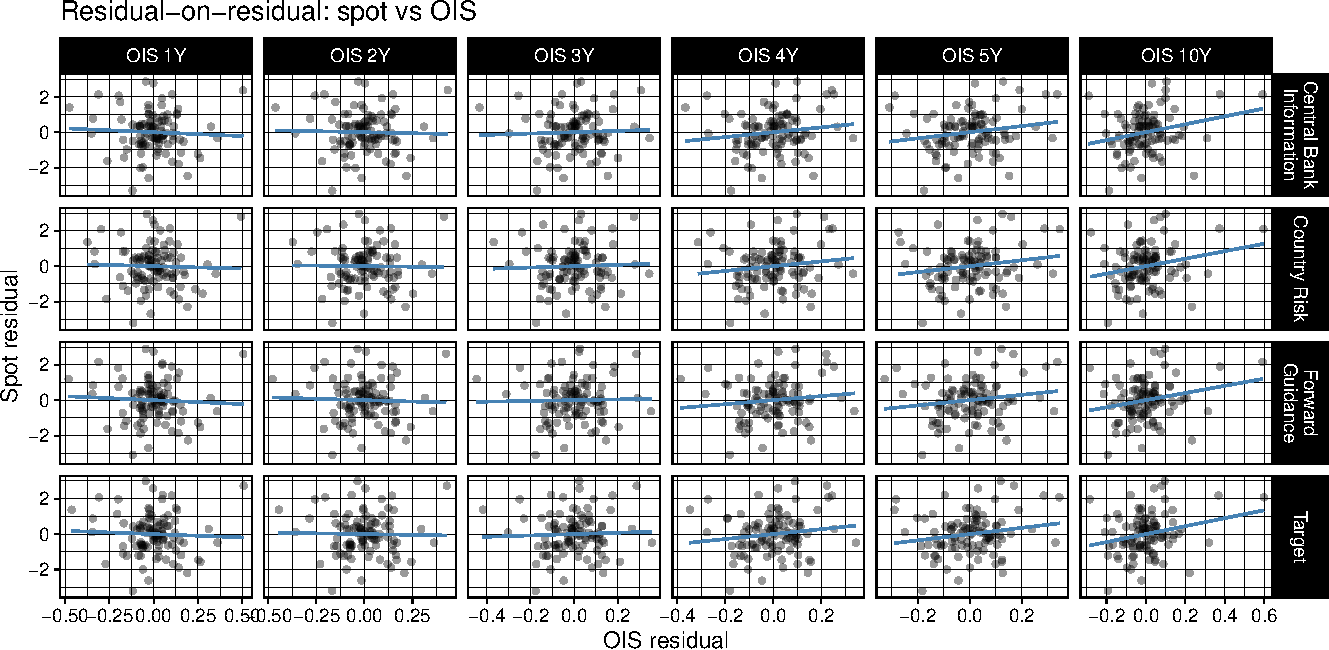
\includegraphics[width=1\textwidth,height=0.78\textheight]{exchange_rate_response_to_news_presentation_files/figure-beamer/residual-fig-1.pdf}
\end{center}

\begin{itemize}
\tightlist
\item
  After removing the surprise from both series, spot and gap residuals
  do not co-move: 1 of 24 slopes are significant at 10\%
\end{itemize}
\end{frame}

\section{Dynamic responses}\label{dynamic-responses}

\begin{frame}{Local projections}
\phantomsection\label{local-projections}
\begin{itemize}
\tightlist
\item
  Smooth local projections of each response on each surprise, one shock
  at a time
\item
  Responses are scaled to a \textbf{1 pp} surprise, with 80\% confidence
  bands
\item
  Horizon is counted in \textbf{announcement events}, not days: horizon
  0 is the announcement-day response
\item
  Later horizons show how subsequent event-day changes relate to the
  shock, not the persistence of the shift
\item
  Question: does a surprise shift the rate gap curve in
  \textbf{parallel}, or \textbf{tilt} it?
\item
  Level: the 2y OIS gap. Slope: the 10y gap minus the 2y gap
\end{itemize}
\end{frame}

\begin{frame}{Parallel shift versus tilt (illustration)}
\phantomsection\label{parallel-shift-versus-tilt-illustration}
\begin{center}
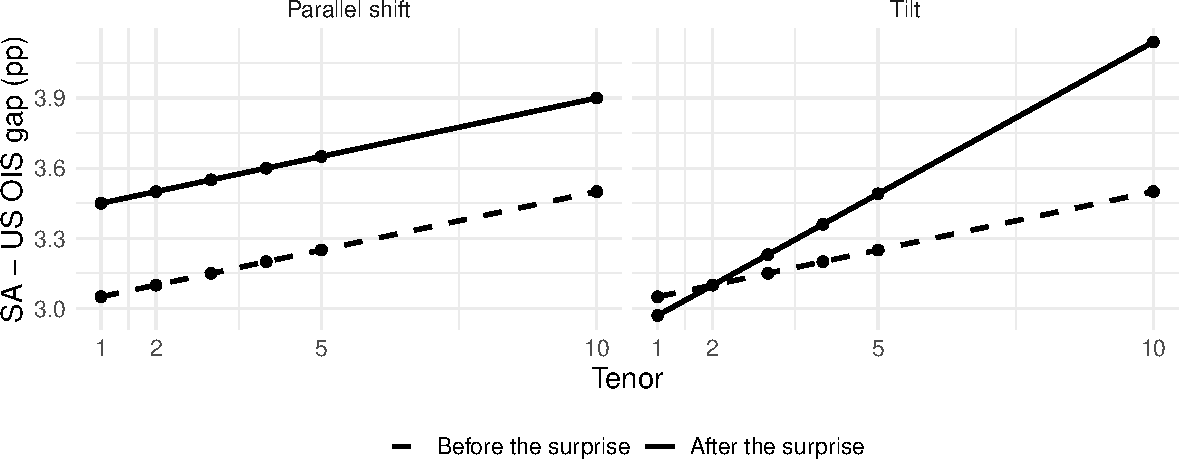
\includegraphics[width=1\textwidth,height=0.55\textheight]{exchange_rate_response_to_news_presentation_files/figure-beamer/tilt-illustration-1.pdf}
\end{center}

\begin{itemize}
\tightlist
\item
  \textbf{Parallel shift:} every tenor moves by the same amount, so the
  level changes and the slope does not
\item
  \textbf{Tilt:} tenors move by different amounts, so the slope changes;
  here the 2y is the pivot and stays put
\item
  We measure the level as the 2y gap response and the slope as the 10y
  minus 2y response (illustrative numbers, not estimates)
\end{itemize}
\end{frame}

\begin{frame}{Spot responses by surprise}
\phantomsection\label{spot-responses-by-surprise}
\begin{center}
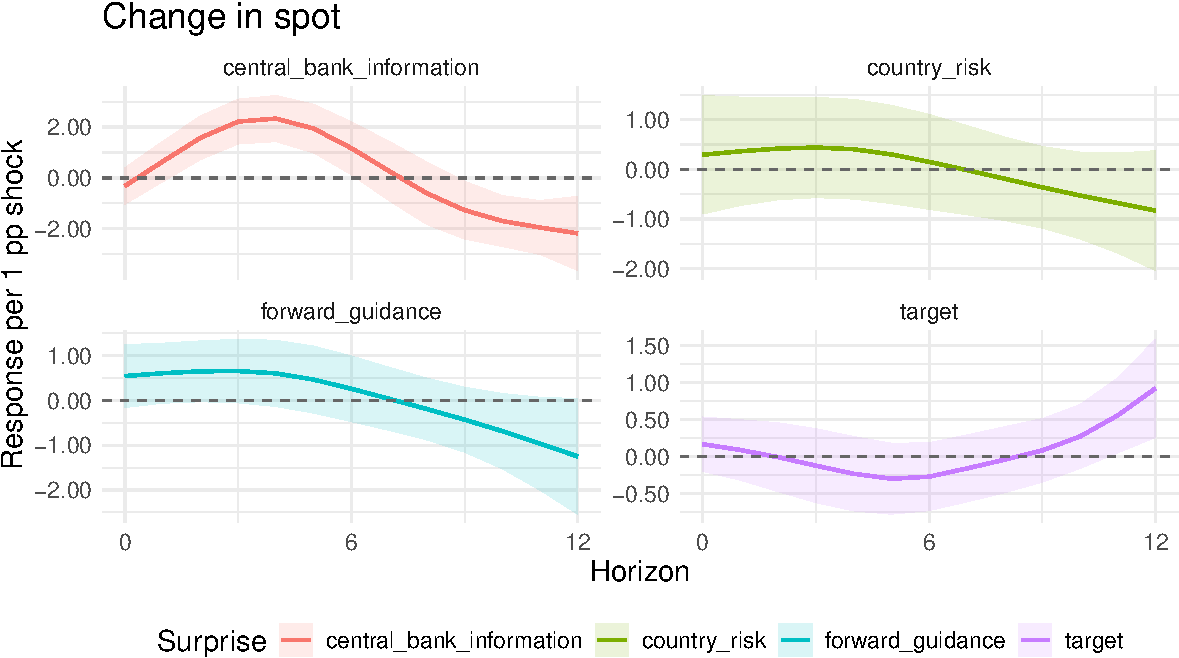
\includegraphics[width=1\textwidth,height=0.78\textheight]{exchange_rate_response_to_news_presentation_files/figure-beamer/lp-spot-1.pdf}
\end{center}
\end{frame}

\begin{frame}{Level: 2y interest gap}
\phantomsection\label{level-2y-interest-gap}
\begin{center}
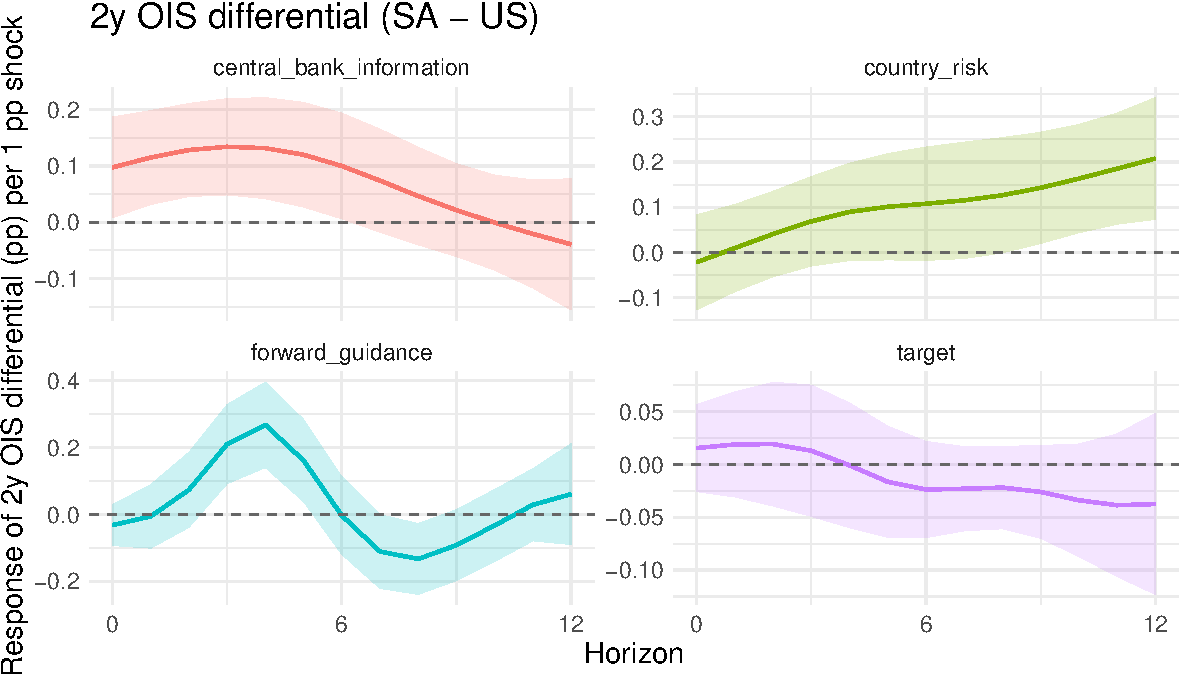
\includegraphics[width=1\textwidth,height=0.78\textheight]{exchange_rate_response_to_news_presentation_files/figure-beamer/lp-level-1.pdf}
\end{center}
\end{frame}

\begin{frame}{Slope: 10y minus 2y interest gap}
\phantomsection\label{slope-10y-minus-2y-interest-gap}
\begin{center}
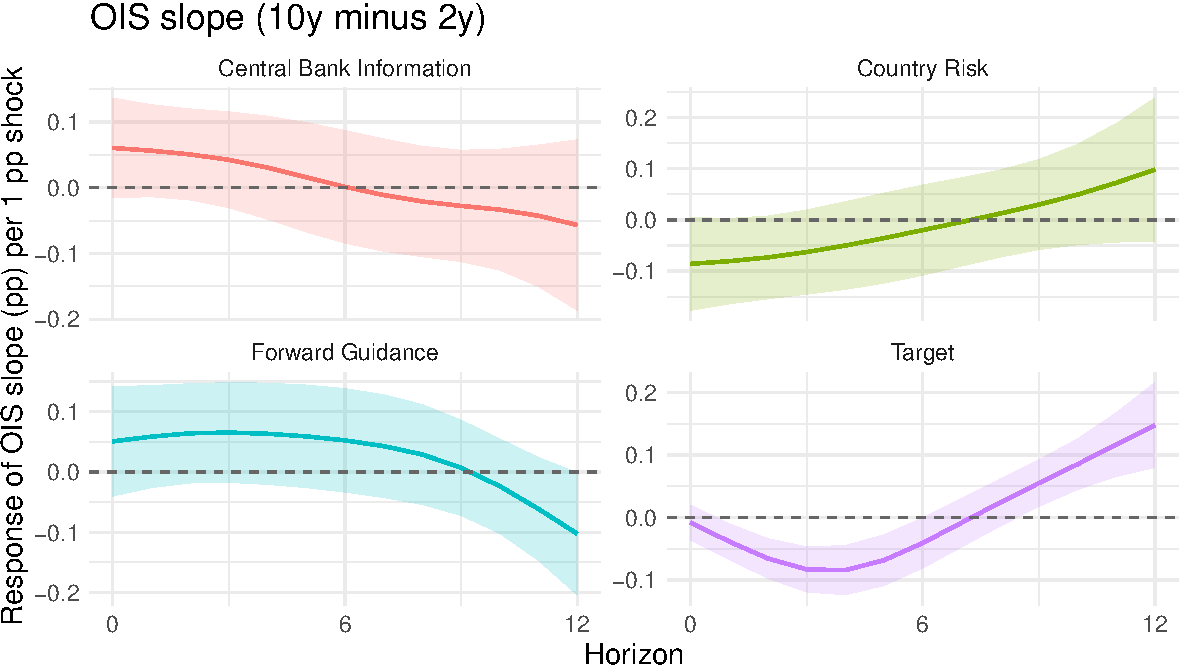
\includegraphics[width=1\textwidth,height=0.78\textheight]{exchange_rate_response_to_news_presentation_files/figure-beamer/lp-slope-1.pdf}
\end{center}
\end{frame}

\begin{frame}{Parallel shift or tilt?}
\phantomsection\label{parallel-shift-or-tilt}
\begin{itemize}
\tightlist
\item
  \textbf{CBI} and \textbf{forward guidance} move the 2y gap with little
  change in the slope: closer to a parallel shift
\item
  The \textbf{target} surprise barely moves the 2y gap but changes the
  slope: a tilt, with the long end doing the moving
\item
  \textbf{Country risk} shows little response until late horizons
\item
  A zero slope response is consistent with a parallel shift, but only if
  the level moves
\end{itemize}
\end{frame}

\section{Conclusion}\label{conclusion}

\begin{frame}{Storyline - what are we saying?}
\phantomsection\label{storyline---what-are-we-saying}
\begin{enumerate}
\tightlist
\item
  \textbf{SA monetary policy moves the rand, but not through the gap.}
  Target and FG move spot (-0.99 (p = 0.056) and -2.60 (p = 0.076)),
  while the gap responds to CBI and country risk instead
\item
  \textbf{Domestic macro news moves rates, and growth news also moves
  the rand.} A CPI surprise raises the gap (2y: 0.24 (p \textless{}
  0.001)); a GDP surprise raises the gap and strengthens the rand (-0.64
  (p = 0.001))
\item
  \textbf{US policy transmits through the gap.} US forward guidance
  narrows the gap (2y: -0.05 (p \textless{} 0.001)) and weakens the rand
  (0.35 (p = 0.011))
\item
  \textbf{The gap is a poor day-to-day explanation of the rand.} Raw gap
  changes explain almost none of the variation in spot (R-squared at
  most 0.05)
\end{enumerate}
\end{frame}

\begin{frame}{Caveats and next steps}
\phantomsection\label{caveats-and-next-steps}
\begin{itemize}
\tightlist
\item
  Small sample of announcement days and borderline significance, with no
  correction for multiple tests
\item
  Forwards are implied by CIP and add no independent information;
  observed forwards would allow a \textbf{CIP deviation} analysis
\item
  Local projection results can be sensitive to lag length, and horizons
  are in event time
\item
  Level is proxied by the 2y gap; an average across tenors would
  separate level and slope more cleanly (debatable)
\end{itemize}
\end{frame}

\begin{frame}{The End}
\phantomsection\label{the-end}
\vfill
\begin{center}
\Huge Thank you
\end{center}
\vfill
\end{frame}

\section{References}\label{references}

\begin{frame}[allowframebreaks]{References}
\small

\phantomsection\label{refs}
\begin{CSLReferences}{1}{0}
\bibitem[\citeproctext]{ref-andersen2003}
Andersen, Torben G., Tim Bollerslev, Francis X. Diebold, and Clara Vega.
2003. {``Micro {Effects} of {Macro Announcements}: {Real-Time Price
Discovery} in {Foreign Exchange}.''} \emph{American Economic Review} 93
(1): 38--62.

\bibitem[\citeproctext]{ref-clarida2008}
Clarida, Richard H., and Daniel Waldman. 2008. {``Is Bad News about
Inflation Good News for the Exchange Rate? {And}, If so, Can That Tell
Us Anything about the Conduct of Monetary Policy?''} In \emph{Asset
Prices and Monetary Policy}, 371--96. University of Chicago Press.

\bibitem[\citeproctext]{ref-coleman2012}
Coleman, Andrew, and Özer Karagedikli. 2012. {``The Relative Size of
Exchange Rate and Interest Rate Responses to News: {An} Empirical
Investigation.''} \emph{The North American Journal of Economics and
Finance} 23 (1): 1--19.

\bibitem[\citeproctext]{ref-cook1989}
Cook, Timothy, and Thomas Hahn. 1989. {``The Effect of Changes in the
Federal Funds Rate Target on Market Interest Rates in the 1970s.''}
\emph{Journal of Monetary Economics} 24 (3): 331--51.

\bibitem[\citeproctext]{ref-engel2007}
Engel, Charles, Nelson C. Mark, Kenneth D. West, Kenneth Rogoff, and
Barbara Rossi. 2007. {``Exchange {Rate Models Are Not} as {Bad} as {You
Think} {[}with {Comments} and {Discussion}{]}.''} \emph{NBER
Macroeconomics Annual} 22 (January): 381--473.
\url{https://doi.org/10.1086/ma.22.25554969}.

\bibitem[\citeproctext]{ref-engel2004}
Engel, Charles, and Kenneth D. West. 2004. {``Taylor {Rules} and the
{Deutschmark-Dollar Real Exchange Rate}.''} Working \{\{Paper\}\} 10995.
National Bureau of Economic Research.

\bibitem[\citeproctext]{ref-engel2005}
---------. 2005. {``Exchange {Rates} and {Fundamentals}.''}
\emph{Journal of Political Economy} 113 (3): 485--517.
\url{https://doi.org/10.1086/429137}.

\bibitem[\citeproctext]{ref-faust2003}
Faust, Jon, John H. Rogers, Shing-Yi B. Wang, and Jonathan H. Wright.
2003. {``The {High-Frequency Response} of {Exchange Rates} and {Interest
Rates} to {Macroeconomic Announcements}.''} International \{\{Finance
Discussion Papers\}\} 784. Board of Governors of the Federal Reserve
System.

\bibitem[\citeproctext]{ref-gurkaynak2005a}
Gurkaynak, Refet S, Brian Sack, and Eric T Swanson. 2005. {``Do {Actions
Speak Louder Than Words}? {The Response} of {Asset Prices} to {Monetary
Policy Actions} and {Statements}.''} \emph{International Journal of
Central Banking} 1 (1).

\bibitem[\citeproctext]{ref-gurkaynak2005d}
Gürkaynak, Refet S, Brian Sack, and Eric Swanson. 2005. {``The
{Sensitivity} of {Long-Term Interest Rates} to {Economic News}:
{Evidence} and {Implications} for {Macroeconomic Models}.''}
\emph{American Economic Review} 95 (1): 425--36.
\url{https://doi.org/10.1257/0002828053828446}.

\bibitem[\citeproctext]{ref-jarocinski2024a}
Jarociński, Marek. 2024. {``Estimating the {Fed}'s Unconventional Policy
Shocks.''} \emph{Journal of Monetary Economics} 144: 103548.

\bibitem[\citeproctext]{ref-karagedikli2008}
Karagedikli, Özer, and Pierre L. Siklos. 2008. {``Explaining {Movements}
in the {NZ Dollar}: {Central Bank Communication} and the {Surprise
Element} in {Monetary Policy}?''} Discussion \{\{Paper\}\} DP2008/02.
Reserve Bank of New Zealand.

\bibitem[\citeproctext]{ref-kearns2005}
Kearns, Jonathan, and Phil Manners. 2005. {``Results\textbar{} {RDP}
2005-02: {The Impact} of {Monetary Policy} on the {Exchange Rate}: {A
Study Using Intraday Data}.''} \emph{Reserve Bank of Australia Research
Discussion Papers}, no. December.

\bibitem[\citeproctext]{ref-kuttner2001b}
Kuttner, Kenneth N. 2001. {``Monetary Policy Surprises and Interest
Rates: {Evidence} from the {Fed} Funds Futures Market.''} \emph{Journal
of Monetary Economics} 47 (3): 523--44.

\bibitem[\citeproctext]{ref-lunsford2020}
Lunsford, Kurt G. 2020. {``Policy {Language} and {Information Effects}
in the {Early Days} of {Federal Reserve Forward Guidance}.''}
\emph{American Economic Review} 110 (9): 2899--2934.
\url{https://doi.org/10.1257/aer.20181721}.

\bibitem[\citeproctext]{ref-miranda-agrippino2021}
Miranda-Agrippino, Silvia, and Giovanni Ricco. 2021. {``The Transmission
of Monetary Policy Shocks.''} \emph{American Economic Journal:
Macroeconomics} 13 (3): 74--107.

\bibitem[\citeproctext]{ref-pirozhkova2024a}
Pirozhkova, Ekaterina, Giovanni Ricco, and Nicola Viegi. 2024.
{``Trouble Every Day: {Monetary} Policy in an Open Emerging Economy.''}

\bibitem[\citeproctext]{ref-swanson2021a}
Swanson, Eric T. 2021. {``Measuring the Effects of Federal Reserve
Forward Guidance and Asset Purchases on Financial Markets.''}
\emph{Journal of Monetary Economics} 118: 32--53.

\bibitem[\citeproctext]{ref-zettelmeyer2004}
Zettelmeyer, Jeromin. 2004. {``The Impact of Monetary Policy on the
Exchange Rate: Evidence from Three Small Open Economies.''}
\emph{Journal of Monetary Economics} 51 (3): 635--52.

\end{CSLReferences}
\end{frame}

\section{Appendix}\label{appendix}

\begin{frame}{South African monetary policy surprises}
\phantomsection\label{south-african-monetary-policy-surprises}
\begin{center}
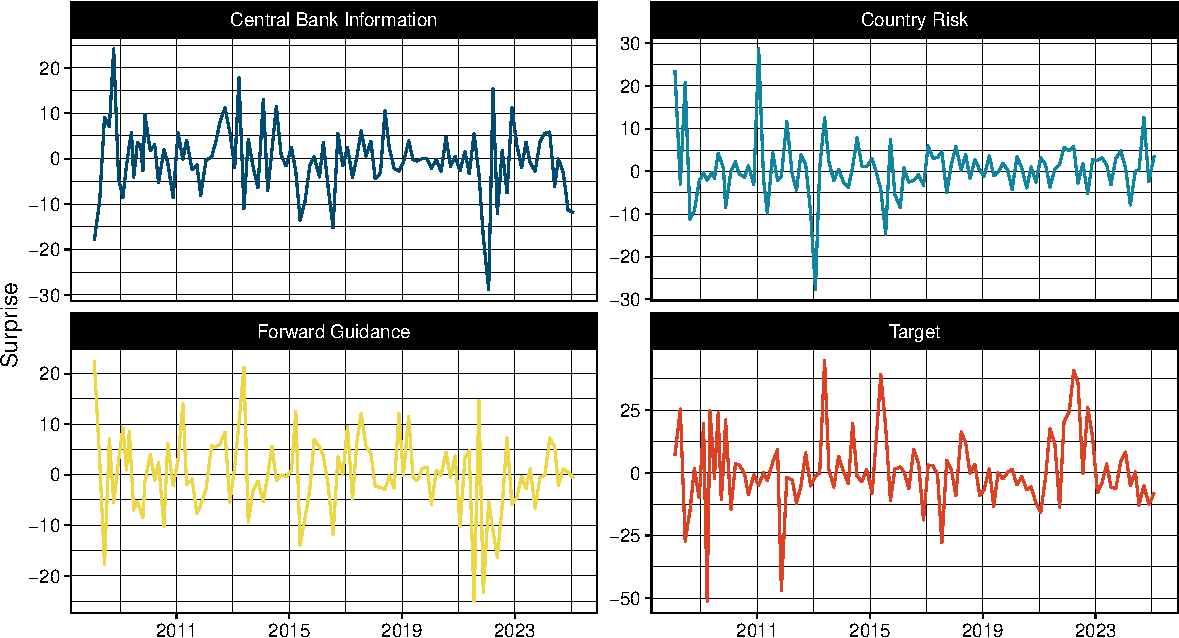
\includegraphics[width=1\textwidth,height=0.78\textheight]{exchange_rate_response_to_news_presentation_files/figure-beamer/sa-surprises-1.pdf}
\end{center}
\end{frame}

\begin{frame}{US monetary policy surprises: data}
\phantomsection\label{us-monetary-policy-surprises-data}
\begin{center}
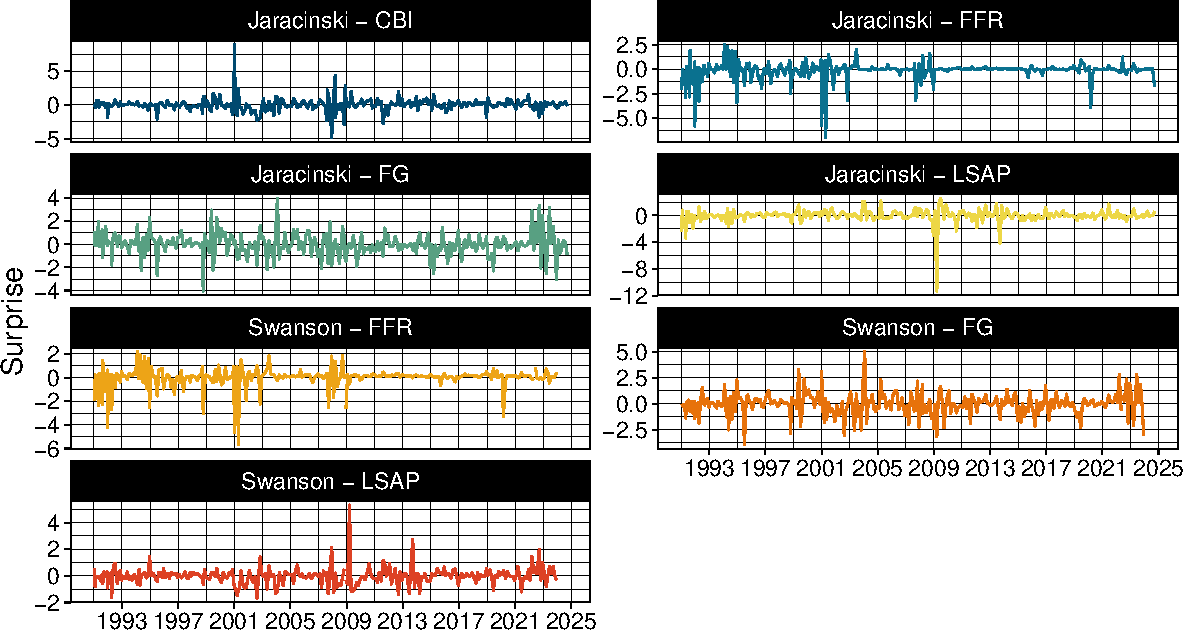
\includegraphics[width=1\textwidth,height=0.78\textheight]{exchange_rate_response_to_news_presentation_files/figure-beamer/us-surprises-data-1.pdf}
\end{center}
\end{frame}

\begin{frame}{SA OIS rates}
\phantomsection\label{sa-ois-rates}
\begin{center}
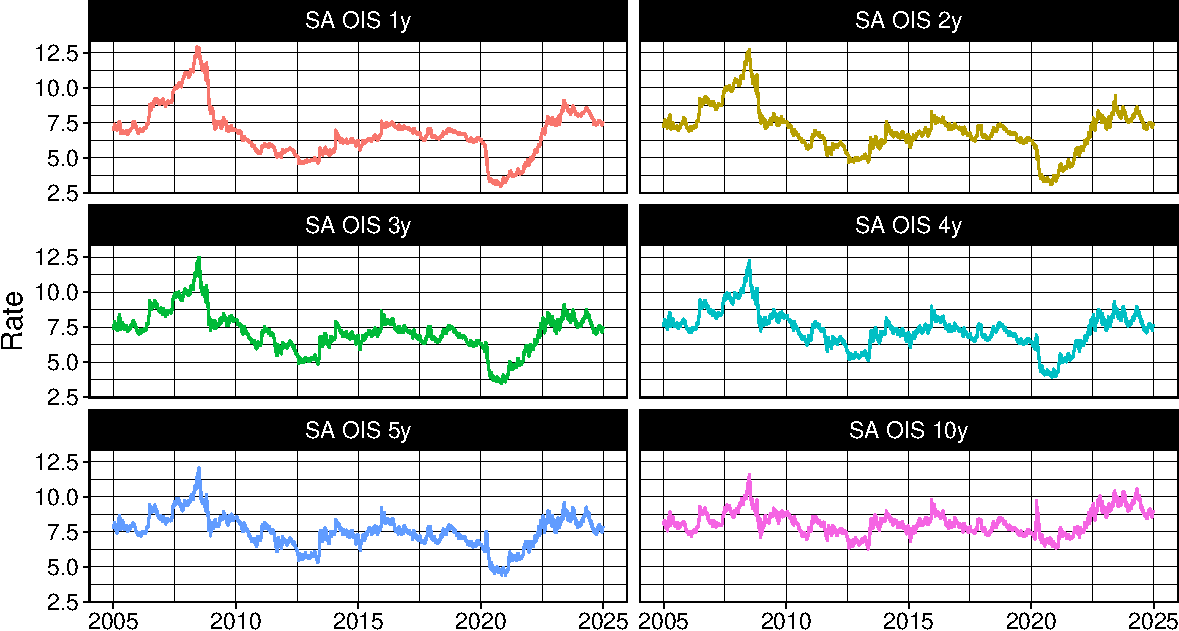
\includegraphics[width=1\textwidth,height=0.78\textheight]{exchange_rate_response_to_news_presentation_files/figure-beamer/zaronia-1.pdf}
\end{center}
\end{frame}

\begin{frame}{Forward responses to SA monetary policy surprises}
\phantomsection\label{forward-responses-to-sa-monetary-policy-surprises}
\begin{center}
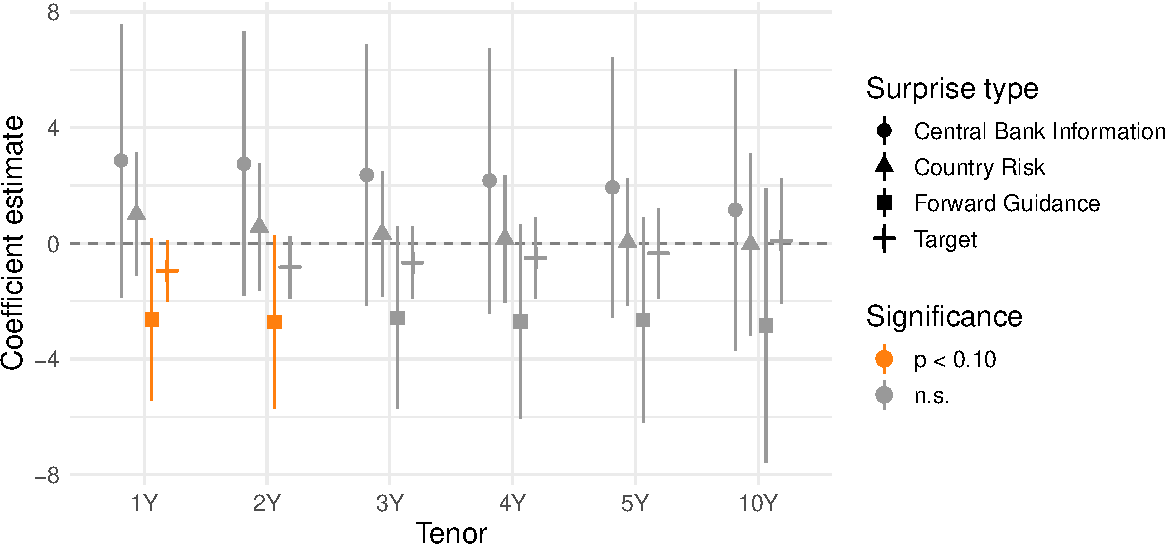
\includegraphics[width=1\textwidth,height=0.62\textheight]{exchange_rate_response_to_news_presentation_files/figure-beamer/forward-responses-1.pdf}
\end{center}

\begin{itemize}
\tightlist
\item
  Forwards are built as spot plus n times the change in the gap, so they
  carry no independent information
\item
  At short tenors they mirror the spot response; the gap component grows
  with the tenor
\item
  Shown for the SA monetary policy surprises only
\end{itemize}
\end{frame}

\begin{frame}{Descriptive statistics}
\phantomsection\label{descriptive-statistics}
\begin{table}[!h]
\centering\begingroup\fontsize{7}{9}\selectfont

\resizebox{\ifdim\width>\linewidth\linewidth\else\width\fi}{!}{
\begin{tabular}[t]{lrrrrrr}
\toprule
Series & Mean & Median & SD & Min & Max & Observations\\
\midrule
Forward 10y & 0.027 & -0.039 & 1.776 & -12.036 & 17.721 & 4,137\\
Forward 1y & 0.024 & -0.023 & 1.155 & -10.665 & 16.341 & 4,137\\
Forward 2y & 0.024 & -0.023 & 1.194 & -10.993 & 16.557 & 4,137\\
Forward 3y & 0.024 & -0.021 & 1.249 & -10.956 & 16.653 & 4,137\\
Forward 4y & 0.024 & -0.012 & 1.312 & -10.983 & 16.780 & 4,137\\
Forward 5y & 0.024 & -0.020 & 1.382 & -10.775 & 17.009 & 4,137\\
Spot & 0.025 & 0.000 & 1.137 & -10.232 & 16.213 & 4,137\\
OIS gap 10y & 0.000 & -0.002 & 0.102 & -0.583 & 0.759 & 4,137\\
OIS gap 1y & -0.001 & -0.002 & 0.069 & -0.595 & 0.664 & 4,137\\
OIS gap 2y & -0.000 & -0.003 & 0.086 & -0.834 & 0.700 & 4,137\\
OIS gap 3y & -0.000 & -0.002 & 0.092 & -0.570 & 0.645 & 4,137\\
OIS gap 4y & -0.000 & -0.002 & 0.096 & -0.591 & 0.662 & 4,137\\
OIS gap 5y & -0.000 & -0.002 & 0.099 & -0.563 & 0.661 & 4,137\\
\bottomrule
\end{tabular}}
\endgroup{}
\end{table}
\end{frame}



\end{document}
